%%%%%%%%%%%%%%%%%%%%%%%%%%%%%%%%%%%%%%%%%%%%%%%%%%%%%%%%%%%%%%%%%%%%%%%%%%%%%%%%%%%%%
%																					%
%	TRABAJO: Proyecto Integrador													%
%																					%
%		Titulo: 	Desarrollo de IP cores con procesamiento de Redes de Petri 		%
%					Temporales para sistemas multicore en FPGA						%
%																					%
%		Autores:	Juli�n Nonino													%
%					Carlos Renzo Pisetta											%
%		Director:	Orlando Micolini												%
%																					%
%	Parte: Marco Teorico															%
%	Capitulo: Redes de Petri														%
%	Seccion: Propiedades de las Redes de Petri										%	
%	Archivo: propiedades.tex														%
%																					%
%%%%%%%%%%%%%%%%%%%%%%%%%%%%%%%%%%%%%%%%%%%%%%%%%%%%%%%%%%%%%%%%%%%%%%%%%%%%%%%%%%%%%

% Path Imagenes: ./marco_teorico/redes_de_petri/img
% Nombre predeterminado imagenes: petrixx
%	xx es el numero de imagen

\section{Propiedades de las Redes de Petri}
	\label{sec:propiedades_petri}

	Las Redes de Petri tienen propiedades especiales que se detallar�n a continuaci�n.
	
	\subsection{Redes de Petri limitadas}
		
		Sea la Red de Petri $PN = {P, T, I^-, I^+, m_0}$, se dice que una plaza $p$ es \textbf{\emph{k-limitada}}
		si existe un valor $k$ tal que para todo marcado $m$ perteneciente al conjunto de marcados de la Red de 
		Petri $PN$ se cumple que el valor de marcado de la plaza $p$ es menor o igual que $k$.
		\begin{equation}
			\exists k / \forall m \in marcados(PN) : m(p) \leq k
			\label{eq:red_limitada}
		\end{equation}
		
		El arreglo $marcados(PN)$ representa todos los marcados posibles de la Red de Petri.
		
		Se dice que una Red de Petri es \emph{k-limitada} si todas sus plazas son \emph{k-limitadas}.
		
	\subsection{Redes de Petri seguras}
	
		Se dice que una red de Petri PN es \textbf{\emph{segura}} si y s�lo si todas sus plazas son \textbf{\emph{1-limitadas}}.
		Esto implica que una transici�n no puede ser disparada si alguna de sus plazas de llegada est� ocupada.
		
	\subsection{Redes de Petri c�clicas}
			
		Se dice que una Red de Petri es \textbf{\emph{c�clica}} si existe siempre una sucesi�n de marcados que 
		lleve desde cualquier marcado $m$ al marcado inicial $m_0$.
	
	\subsection{Redes de Petri repetitivas}

		Se dice que una Red de Petri es \textbf{\emph{repetitiva}} si existe siempre una secuencia de disparos que 
		lleve desde un marcado $m$ hasta el mismo marcado $m$.

	\subsection{Redes de Petri conservativas}

		Una Red de Petri es \textbf{\emph{conservativa}} si se cumple que para todo marcado $m$ perteneciente 
		al conjunto de marcados de la red, la cantidad de marcas de $m$ es igual a la cantidad de marcas de 
		$m_0$. Es decir, se conserva la cantidad de tokens.

	\subsection{Propiedad de vivacidad (liveness)}

		Se dice que una Red de Petri esta \textbf{\emph{viva}} si y s�lo si en todo momento sus transiciones 
		pueden ser disparadas o si existe una secuencia de disparos v�lidos que lleven a que la transici�n 
		pueda dispararse. 

	\subsection{Propiedades de bloqueo (deadlock)}
	
		Un \textbf{\emph{bloqueo}} en una Red de Petri implica que una transici�n nunca podr� ser disparada 
		independientemente de la secuencia de disparos que se aplique.
		
		Recordando la propiedad anterior, se puede decir que una Red de Petri viva garantiza la ausencia de 
		bloqueos.
		
		Este concepto est� sustentado en la ausencia de \emph{marcados sumideros}. Un marcado sumidero es 
		aquel marcado a partir del cual ninguna transici�n puede ser disparada.
		
	\subsection{Alcanzabilidad}

		La alcanzabilidad determina si un marcado $m$ es alcanzable desde un marcado inicial $m_0$, es 
		decir, determina si $m$ pertenece al conjunto de marcados de la Red de Petri.
		
		Se dice que un marcado $m$ es alcanzable desde $m_0$ si y s�lo si existe una secuencia de disparos 
		que lleven desde $m_0$ hasta $m$.
		
		Para determinar si un marcado $m$ es alcanzable, se utiliza la ecuaci�n de estado de una Red de 
		Petri de la siguiente manera:
		\begin{equation}
			m = m_0 + I � \sigma
			\label{eq:alcanzabilidad}
		\end{equation}
		D�nde $\sigma$ es una secuencia de disparos.
				
		Si no fuera posible encontrar una secuencia de disparos, se dice que el marcado $m$ es \emph{inalcanzable}.
		
		Si existieran m�ltiples soluciones, es decir, varias secuencias de disparos posibles para 
		alcanzar el marcado $m$, se dice que la Red de Petri se comporta de manera \emph{NO determin�stica}.
		
		Hay que notar que la soluci�n de la ecuaci�n no indica el orden en que las transiciones deben ser 
		disparadas, por lo que, �ste debe ser encontrado ejecutando todas las secuencias posibles. Por ello, es 
		posible que a pesar de encontrar una secuencia de disparos, no exista un ordenamiento de los mismos que 
		permita alcanzar la marca $m$ y sea aplicable a la Red de Petri en cuesti�n.
		
		\subsubsection{Grafo de alcanzabilidad}
				
			El grafo de alcanzabilidad de una Red de Petri representa el conjunto de todos los marcados 
			alcanzables desde el marcado inicial $m_0$. Consiste en un grafo en forma de �rbol en el que 
			cada nodo es un marcado alcanzable de la red y se conectan mediante arcos etiquetados con la 
			transici�n que se dispara para pasar de un marcado a otro.
			
			Partiendo del estado inicial $m_0$ se generan todos los estados alcanzables desde �ste mediante 
			un disparo de cada una de las transiciones sensibilizada. A partir de cada estado, se vuelve a 
			repetir el proceso, apareciendo, en consecuencia, un grafo en forma de �rbol que representa todos 
			los estados del sistema.
			
			Por ejemplo, sea la siguiente Red de Petri, se plantear� el grafo de alcanzabilidad de la misma.
				
			\begin{figure}[H]
				\centering
				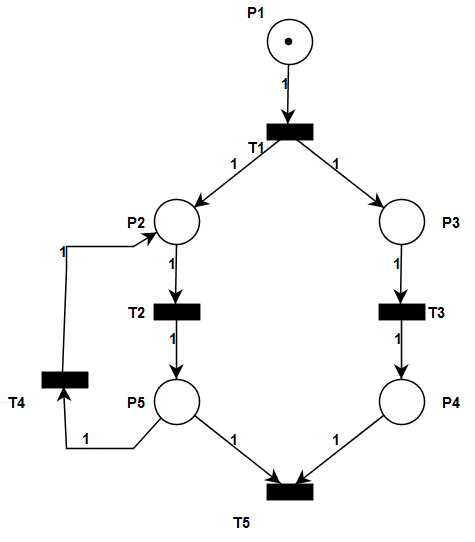
\includegraphics[width=0.5\linewidth]{./marco_teorico/redes_de_petri/img/Petri02}
				\caption{Red de Petri de Ejemplo para Grafo de alcanzabilidad}
				\label{fig:Petri02}
			\end{figure}
				
			El grafo de alcanzabilidad de la red de la Figura \ref{fig:Petri02}, comenzar�a de la siguiente 
			manera:
			\begin{figure}[H]
				\centering
				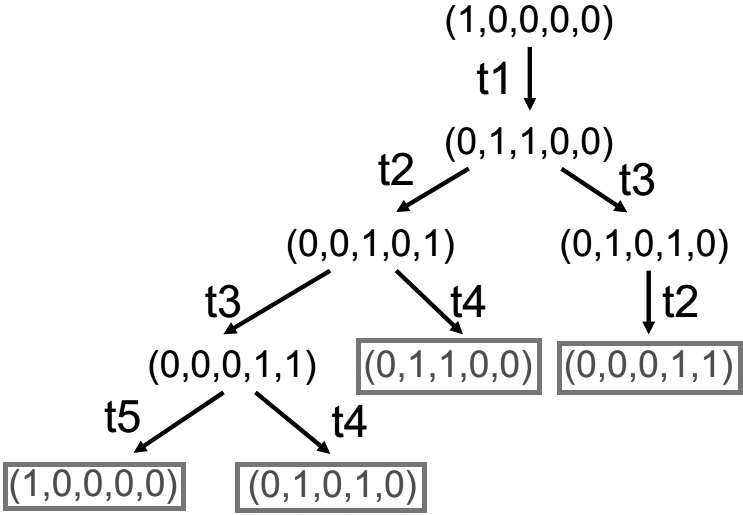
\includegraphics[width=0.65\linewidth]{./marco_teorico/redes_de_petri/img/Petri03}
				\caption{Ejemplo de grafo de alcanzabilidad}
				\label{fig:Petri03}
			\end{figure}
			El proceso se detiene en los marcados repetidos, que en la Figura \ref{fig:Petri03} aparecen recuadrados.
				
				
					